\documentclass[a4paper,11pt]{article}

\usepackage{amsmath}
\usepackage{amssymb}
\usepackage{amsthm}
\usepackage{graphicx}
\usepackage{enumerate}
\usepackage{xcolor}
\usepackage{biblatex}
\usepackage{rotating}
\usepackage{algorithm}
\usepackage{algpseudocode}
\usepackage{pdflscape}
\usepackage[hidelinks]{hyperref}
\hypersetup{
    colorlinks=false, %set true if you want colored links
    linktoc=all,     %set to all if you want both sections and subsections linked
    linkcolor=black,  %choose some color if you want links to stand out
}


\addbibresource{percolation.bib}

%------------------

%\setlength{\topmargin}{0.0in}
%\setlength{\textheight}{10in}
%\setlength{\oddsidemargin}{0.0in}
%\setlength{\evensidemargin}{0.0in}
%\setlength{\textwidth}{6.5in}

%-------------------
\newtheorem{theorem}{Theorem}[section]
\newtheorem{proposition}[theorem]{Proposition}
\newtheorem{lemma}[theorem]{Lemma}
\newtheorem{corollary}[theorem]{Corollary}
\newtheorem{conjecture}[theorem]{Conjecture}


\theoremstyle{definition}
\newtheorem{definition}[theorem]{Definition}
\newtheorem*{example}{Example}
\newcommand{\ints}{\mathbb{Z}}
\newcommand{\sigalg}{$\sigma$-algebra }
\newcommand{\ztwodual}{(\ints^2)^*}
\newcommand{\prob}{\mathbb{P}_p}
\newcommand{\expp}{\mathbb{E}_p}
%------------------

%Everything before begin document is called the pre-amble and sets out how the document will look
%It is recommended you don't touch the pre-amble until you are familiar with LaTeX

\begin{document}
\thispagestyle{empty}

\begin{figure}[h]
\begin{center}

\includegraphics[scale=0.5]{uob.pdf} %make sure the pdf file named 'uob' is saved in the same folder as this file
\end{center}
\end{figure}

\begin{center}
{\Large Percolation\\ \vspace{1cm}Jonathan Marriott}
\end{center}

\vspace{3cm}
\hrule
\begin{center}
Supervised by Dr Edward Crane\\
Level 6\\
20 Credit Points
\end{center}
\hrule

\vspace{3cm}
\begin{center}
\today
\end{center}
	
\title{Percolation}
\author{Jonathan Marriott}
\date{}
\maketitle

% \begin{abstract}
% Some sorts of documents need abstracts. Others do not.
% \end{abstract}

%The following code is not run because of the percentage sign, but you might find it useful for future work
\tableofcontents{}


\section{Introduction}

A project on Percolation 
%Using the percentage symbol, you can include comments in your code that do not appear in the output.


% \section{Formatting}

% We can \emph{emphasis} some words, i.e., make them \emph{italic}, and we can make some words \textbf{bold}.
% Note how using a new line in the code does not correspond to a new line in the output file.
% Same if we have        a           large                white                   space.

% Instead, if we want a new line/new paragraph, you need to press enter twice, or use \\
% which starts a new line but not a new paragraph.

% \subsection{lists}

% Lists can be numbered or unnumbered, and you can have sub-list inside a list.

% \begin{enumerate}
% 	\item This is the first item in a numbered list.

% 	\item And the second
	
% 	\item 
% 	\begin{enumerate}
% 		\item Here the third item is in fact a numbered sub-list.
% 		\item item 2 of the numbered sub-list
% 	\end{enumerate}

% 	\item 
% 	\begin{itemize}
% 		\item Here the fourth item is an unnumbered sub-list.
% 		\item item 2 of the unnumbered sub-list
% 	\end{itemize}
% \end{enumerate}
\section{The Percolation Model}
\subsection{Initial Definitions}

We start with some basic definitions for Percolation on cubic lattices, specifically bond percolation where we consider the edges on the graph to be either open or closed. 

\begin{definition}\label{ints} 
	$\mathbb{Z} = \{...,-2,-1,0,1,2,...\}$ and $\mathbb{Z}^d = \{(x_1,x_2,...,x_d) : x_i \in \mathbb{Z} \}$
\end{definition}

\begin{definition}\label{dist}
	For $x,y\in \mathbb{Z}^d$, define the distance from x to y, denoted $\delta(x,y)$, by
	$$\delta(x,y) := \sum_{i=1}^{d}|x-y|$$
\end{definition}\label{lattice} 

\begin{definition}[d-dimensional cubic lattice]{
	We construct the lattice with vertices in $\ints^d$ and edges where the distance between vertices is one.
	$$E(\ints^d) = \{\{u,v\}:u,v \in V(\ints^d),\: \delta(u,v) = 1\}$$
	We will often refer to this lattice by the vertex set $\ints^d$ without specifying the edge set.
	We also denote the origin by 0.
}
\end{definition}


\subsection{Probability Space}

We now introduce the Measure theory basics required to define the probability measure and subsequently the probability space for our percolation model.

\begin{definition}[$\sigma$-algebra]
	For some set $X$, we call $\mathcal{A} \subseteq \mathcal{P}(X)$, a subset of the power set of X, a  $\sigma$-algebra of $X$ if:
	\begin{enumerate}
		\item $\emptyset,X \in \mathcal{A}$
		\item $A \in \mathcal{A} \implies A^c := X \setminus A \in \mathcal{A}$ (Closed under complement)
		\item For $A_i \in \mathcal{A}, i \in \mathbb{N}$ we have that $\bigcup^\infty_{i=1} A_i \in \mathcal{A}$ (Closed under countable unions)
	\end{enumerate}
	We call the pair $(X,\mathcal{A})$ a measurable space, and elements of $\mathcal{A}$ measurable sets.
\end{definition}

We note by De Morgan's Laws that a $\sigma$-algebra is also closed under countable intersections.

\begin{definition}[Measure]
	A measure $\mu$ on a measurable space $(X,\mathcal{A})$ is a function $\mu: \mathcal{A} \rightarrow [0,\infty]$ where 
	$\mu(\emptyset) = 0 $ and for disjoint $A_i \in \mathcal{A}, i \in \mathbb{N}$ we have that
	$$ \mu(\bigcup^\infty_{i=1} A_i) = \sum_{i = 1}^{\infty} \mu(A_i)  $$
	We call the triple $(X,\mathcal{A},\mu)$ a measure space.
\end{definition}

In the context above if we think about X being our set of outcomes, and the sigma algebra of X representing the set of events we wish to assign a probability to, it's intuitive to give these events a probability by a measure. 
Clearly we need to restrict our probability measure such that its domain is the interval $[0,1]$ 

\begin{definition}[Probability Measure]
	Let $\Omega$ be the set of all outcomes (the sample space) and $\mathcal{F}$ be a \sigalg of $\Omega$ where the elements are events we wish to consider (the event space). Then a measure $\mathbb{P}$ on $(\Omega,\mathcal{F})$ is a probability measure if:
	\begin{enumerate}
		\item $\mathbb{P}: \mathcal{F} \rightarrow [0,1]$
		\item $\mathbb{P}(\Omega) = 1$
	\end{enumerate}
	Then we call the triple $(\Omega,\mathcal{F},\mathbb{P})$ a probability space.
	
\end{definition}

\subsection{The Model}

We now take some $p \in [0,1]$ which will be our parameter which specifies the probability a given edge is open. 
Setting $q = 1-p$ we say each edge is independently open with probability p and closed with probability q.
We can think of the open and closed edges defining a random subgraph of $\ints^d$ where only edges set to open are retained.\\

We let our sample space $\Omega = \prod_{e \in E} \{0,1\}$ where $E = E(\ints^d)$ and an edge in state 1 represents it is open, and 0 that it is closed.\\
We may refer to $\Omega$ as the set of configurations, where a configuration $\omega$ is a function assigning edges to be open or closed, meaning 
$$\omega:E \to \{0,1\}, e \mapsto \omega_e$$
Then we must define $\mathcal{F}$, some \sigalg of $\Omega$, the events we wish to assign a probability to. 
Clearly we cannot just take $\mathcal{F} = \mathcal{P}(\Omega)$, since we have uncountably many configurations in $\Omega$. 
This can be easily seen via a diagonalization argument. 
It turns out we can generate the \sigalg we want by the cylinder sets of $\Omega$. We base our definition on the one given by \cite{bollo2006}.

\begin{definition}[Cylinder Set]
	We say a subset $S \subseteq \Omega$ is a cylinder set if and only if there exists a finite subset $F \subseteq E$ and $\sigma \in \{0,1\}^F$ such that 
	$$S(F,\sigma) = \{\omega \in \Omega: \omega_f = \sigma_f \text{ for }f \in F\}$$
	In essence the cylinder set is the set of configurations $\omega$ which map all the edges in F to the same state that $\sigma$ does.
\end{definition}

Then we define $\mathcal{F}$ to be the set of all unions of cylinder sets of $\Omega$, then $\mathcal{F}$ is said to be generated by the cylinder sets of $\Omega$.
In this case $\mathcal{F}$ is a \sigalg of $\Omega$. Intuitively $\mathcal{F}$ is the set of events which only depend on a finite number of edges.\\
Next we define our probability measure on $(\Omega, \mathcal{F})$ by 
$$\prob(S(F,\sigma)) = \prod_{f \in F} (p(\sigma_f) + q(1-\sigma_f)) $$
Where as usual $q = 1-p$, and we use the subscript $p$ to emphasize that $p$ is the parameter in our model. 
Notice that we have defined $\prob$ for a cylinder sets rather than elements of the $\sigma$-algebra, however it turns out by
Carathéodory's extension theorem the probability measure above has a unique extension to the whole $\sigma$-algebra.
For the details of this theorem see Theorem 1.3.10 in \cite{ash2000probability}.
Then $(\Omega, \mathcal{F}, \prob)$ is our probability space in which we examine the percolation model.
\\
We now lay out some definitions specific for percolation.
\begin{definition}
	Let $C(x)$ denote the open cluster (component) containing x, which is the set of vertices in $\ints^d$ which are connected to x by a path of open edges.
	We abbreviate the open cluster containing the origin $C(0)$ by $C$
\end{definition}

\begin{definition}[Increasing Event]
	An event $ A \subseteq \Omega$ is increasing if when $\omega \in A$ and
	$$\forall e \in E(\ints^d) \text{, } \omega_e = 1 \implies \omega'_e = 1$$
	Then $\omega' \in A$. 
	\end{definition} 

	We notice that the event $\{|C| = \infty\}$ is clearly an increasing event, since adding open edges to a configuration with an infinite connected cluster containing the origin will not remove the infinite cluster.

\begin{definition}[Percolation function]
	We define the percolation function $\theta(p)$ as follows
	$$\theta(p) = \prob(|C| = \infty)$$
	In words the percolation function is simply the probability that we can reach an infinite number of vertices from the origin by open edges. 
	Furthermore, we also note that this is the same as asking what is the probability of having an infinite length self-avoiding path of open edges starting at the origin.
\end{definition}

We intend to show that this percolation function is non-decreasing, but first we show a more general result for increasing events.

\begin{lemma} \label{incEventlemma}
	If $A \subseteq \Omega$ is an increasing event then $\prob(A)$ is non-decreasing in $p$. 
\end{lemma}

\begin{proof}
	We use the coupling of percolation processes to show that $\prob(A)$ is non-decreasing. We use the definition of couplings given by \cite{roch2015modern}.

	\begin{definition}[Coupling]
		Let $\mathbb{P}$ and $\mathbb{P}'$ be probability measures on the same measurable space $(\Omega,\mathcal{F})$.
		A coupling of $\mathbb{P}$ and $\mathbb{P}'$ is a probability measure $\mathbf{P}$ on $(\Omega\times\Omega,\mathcal{F}\times \mathcal{F})$ such that the marginals of $\mathbf{P}$ coincide with $\mathbb{P}$ and $\mathbb{P}'$.
		Meaning 
		$$\mathbf{P}(A \times \Omega) = \mathbb{P}(A) \quad \text{  and  } \quad \mathbf{P}(\Omega \times A) = \mathbb{P}'(A) \text{, }\quad \forall A \in \mathcal{F}$$
		We say $(X,Y)$ is coupling of $\mathbb{P}$ and $\mathbb{P}'$ for random variables $X,Y$ if the law of $(X,Y)$ is a coupling of $\mathbb{P}$ and $\mathbb{P}'$ as defined above.
	
	\end{definition}

	We construct a pair of configurations $\omega, \omega' \in \Omega$ using a family of uniform random variables $(U_e)_{e\in E}$ which are iid on [0,1].
	Then fixing a pair $p,p' \in [0,1]$ such that $p < p'$, for each $e \in E$ we define its state in $\omega$ by:
	$$\omega_e = \begin{cases}
		1 & \text{if }U_e \leq p\\
		0 & \text{otherwise}\\
	\end{cases} $$
	So each edge in $\omega$ is independently open with probability p. Specifically the law or distribution of $\omega$ is $\prob$ 
	  Similarly define $\omega'$ by:
	$$\omega'_e = \begin{cases}
		1 & \text{if }U_e \leq p'\\
		0 & \text{otherwise}\\
	\end{cases} $$
	Then the law of $\omega'_e$ is $\mathbb{P}_{p'}$. Then since $p \leq p'$ it is clear that
	$$\forall e \in E \text{, }\omega_e \leq \omega'_e $$
	Which we denote by the shorthand $\omega \leq \omega'$.\\
	Then $(\omega,\omega')$ is a coupling of $\mathbb{P}_{p}$ and $\mathbb{P}_{p'}$ with the property that $\mathbf{P}(\omega \leq \omega') = 1$
	Let some increasing event $A \subseteq \Omega$, by definition if $\omega \in A$, then $\omega' \in A$ so:
	$$\mathbb{P}_p(A) = \mathbf{P}(\omega \in A) \leq \mathbf{P}(\omega' \in A) = \mathbb{P}_{p'}(A)$$
	So we conclude $\prob(A)$ is non-decreasing in p

\end{proof}

\begin{corollary}
	The percolation function $\theta(p)$ is non-decreasing in p.
\end{corollary}

\begin{proof}
	Since we already saw that the event $\{|C| = \infty\}$ is an increasing event, then by Lemma \ref{incEventlemma} we know that $\theta(p) = \prob(|C| = \infty)$ is non-decreasing in p.
\end{proof}

An interesting property of our percolation model is that it exhibits a phase transition. Where at some point the behaviour of the model changes notably.
For the percolation model we see there is some value of our parameter $p$, before which we know almost surely there is no infinitely connected cluster, and after which there may be one.
We call this value of $p$ the critical value or percolation threshold.
\begin{definition}[Critical Value]
	We define the critical value $p_c(d)$ formally as follows
	$$p_c(d) = \text{sup}\{p \in [0,1]: \theta(p)=0\} $$
	where d denotes the dimensionality of our graph $\ints^d$, we may sometimes drop the d and just refer to $p_c$ when it is clear what the model dimension is.
\end{definition}



% \begin{definition}\label{my_def}
% 	A \emph{label} allows the user to tell Latex 'remember the numbering of that definition/theorem/equation'
% \end{definition}

% \begin{lemma} \label{my_lem}
% 	If something has a label, then we can refer to it, without knowing what number it is 
% \end{lemma}

% \begin{proof}
% 	For example, by calling up Definition \ref{my_def}. This works even if the ordering of things move.
% 	Note that the end of proof square box is already there
% \end{proof}

% \begin{theorem}
% 	And a final theorem
% \end{theorem}

% \begin{proof}
% 	Combining Definition \ref{my_def} with Lemma \ref{my_lem} we get Equation \ref{my_eqn} below.
% \end{proof}

\section{Existence of a critical value}
\subsection {Existence of a critical value on $\ints$}\label{critvalforZ}
Trivially the critical value is p = 1. Consider the event $X_n = \{$There is an open self-avoiding path of length n starting at the origin$\}$ 
Then $X_n \supseteq X_{n+1}$ and so 
$$\lim_{n\rightarrow \infty} \prob (X_n) = \theta(p)$$
And since $\prob (X_n) = 2p^n$, as the path can go left or right from the origin. We have for all $p <1$, $\theta(p) = 0$. Thus, $\theta(p) > 0$ if and only if $p = 1$. 


\subsection {Existence of a critical value on $\ints^2$}
We show the existence of the critical value in this case by bounding it from above and below. We follow the proofs given in \cite{steif2011mini}
\begin{theorem}
	If $p < 1/3$, $\theta(p) = 0$.
\end{theorem}
\begin{proof}
	Let $X_n = \{$There is an open self-avoiding path of length n starting at the origin$\}$ as in Section \ref{critvalforZ}.
	Then the probability for a path of length n to be open on every edge is $p^n$. The number of paths of length n from the origin is at most $4(3^{n-1})$ since there are 4 edges to choose from at the origin, then for each next step in the path there are at most 3 edges we can pick as the path is self-avoiding.
	Hence, we get $\prob(X_n) \leq  4(3^{n-1})p^n  $. Then we take the limit since
	$\lim_{n\rightarrow \infty}\prob(X_n) = \theta(p)$.
	\begin{align*}
		\lim_{n\rightarrow \infty}\prob(X_n) &\leq  \lim_{n\rightarrow \infty}4(3^{n-1})p^n\\
		 &\leq 4\cdot  3^{-1} \lim_{n\rightarrow \infty}(3p)^{n}
	 \end{align*}
	 Since $p < 1/3$ we have $\theta(p)=\lim_{n\rightarrow \infty}\prob(X_n) = 0$
\end{proof}

\begin{theorem}
	For p close to 1, we have $\theta(p) > 0$
\end{theorem}
\begin{proof}
	We introduce the dual graph $(\ints^2)^*$ which has vertices in $(\ints^2 + \binom{1/2}{1/2} )$, and edges as you would expect between vertices at distance 1.
	Then we can see there is a clear correspondence between the edges of $\ints^2$ and its dual, since each edge in the dual intersects a unique edge in the original graph. 
	Thus, we can create a mapping from the open and closed edges of $\ints^2$ to the dual graph, where the edge in the dual is open if and only if the intersecting edge in $\ints^2$ is closed, and vice versa.\\
	Then we notice that if there exists a cycle of open edges in the dual graph enclosing the origin then the size of the open cluster at the origin is finite. 
	\begin{lemma}\label{originloop}
		$|C| < \infty \iff \exists$ a cycle of open edges in $(\ints^2)^*$  enclosing the origin
	\end{lemma}
	\begin{proof}
		{Thinking visually since there is a ring of open edges in the dual, the open edges from the origin in the original graph cannot extend beyond this ring. A more formal pure graph theory proof can be made but is omitted here.}
	\end{proof}
	Let $X_n = \{$There is a length n cycle of open edges in $\ztwodual$ which surrounds the origin\}
	Then using Lemma \ref{originloop} we see
	$$\prob(|C| < \infty) = \prob(\bigcup_{n=4}^\infty \prob(X_n)) \leq \sum_{n=4}^\infty \prob(X_n) \leq \sum_{n=4}^\infty n \cdot 4(3^{n-1})q^n$$
	Where in the last summation we get $4(3^{n-1})q^n$ as before by counting the number of possible edges a self avoiding walk can take then multiplying by the probability this path is open in the dual graph. 
	We multiply this term by $n$ since we know for every cycle around the origin in the dual there is some smallest $i \in \mathbb{N}$ for which the cycle crosses the edge $\{i,i-1\}$, i.e the positive x-axis. 
	Then we can translate this cycle left and right to the another n positions, this gives up to n new cycles enclosing the origin in the dual graph.\\
	This sum is finite when $q<1/3$, which is when $p>2/3$. 
	We can make the sum arbitrarily small when $p \rightarrow 1$, when the sum is smaller than 1 this implies $\theta(p) > 0$
	Taking the value $p=0.9$ for example, we can calculate, using Wolfram Alpha in this case, that the sum converges to 
	$$\sum_{n=4}^\infty n \cdot 4(3^{n-1})(1-0.9)^n = 0.0683265$$
	Thus $\theta(0.9) > 0$.

\end{proof}
Hence, the critical value $p_c(2) \in (\frac{1}{3},0.9)$




\subsection {Existence of a critical value on $\ints^d$}
We can easily derive the result that $p_c(d)\in (0,1)$ from the previous section. 
We notice that for all $d\geq 2$ we can extract $\ints^d$ from $\ints^{d+1}$ by simply ignoring the extra edges and their states.
Thus, if there exists an infinite open cluster in $\ints^d$ this would also imply there is one in $\ints^{d+1}$.
Since we have just shown $p_c(2) \in (0,1)$ then we must also have $p_c(d) \in (0,1)$ for all d.

{\color{red}{TODO: explain critical value is non-decreasing in d, by coupling argument?}}


\section{Harris-Kesten Theorem}
An important result in percolation theory is that the critical value for the square lattice is $\frac{1}{2}$. 
This result came in two parts, firstly Harris \cite{harris_1960} showed that $p_c(2) \leq \frac{1}{2}$ in 1960.
Then 20 years later Kesten \cite{kesten1980critical} proved $p_c(2) \geq \frac{1}{2}$, these proofs combined resulted in the following theorem.

\begin{theorem}[Harris-Kesten theorem]
	The critical value on $\ints^2$,  $p_c(2) =  \frac{1}{2}$.
\end{theorem}
In this project our aim is to show the Harris part of the theorem, that $p_c(2) \leq \frac{1}{2}$. 
To do this we first introduce some more foundational results.\\

Recall from earlier the definition of an increasing event.
\begin{definition}[Increasing Event]
	An event $ A \subseteq \Omega$ is increasing if when $\omega \in A$ and
	$$\forall e \in E(\ints^d) \text{, } \omega_e = 1 \implies \omega'_e = 1$$
	Then $\omega' \in A$. \\
	\end{definition}
We follow the definitions and proof for the Harris Inequality given by \cite{duminil2018introduction}.
\begin{theorem}[Harris Inequality]
If $A, B \subseteq \Omega$ are increasing events then 
$$\mathbb{P}(A \cap B) \geq \mathbb{P}(A)\mathbb{P}(B)$$
This is a specific case of a more general inequality, the FKG inequality.
If $f$ and $g$ are two bounded increasing functions then
$$ \mathbb{E}_p(fg) \geq \mathbb{E}_p(f)\mathbb{E}_p(g)$$
\end{theorem}
\begin{proof}
	% Suppose some increasing events $A,B \subseteq \Omega$ which only depend on the states of a finite number of edges.
	% Say these edges are $e_1, e_2, ... , e_n$.
	% We work by induction on the size of $n$.\\
	% Consider when $n = 1$, then both $A$ and $B$ just depend on the state of $e_1$. 
	% As both $A$ and $B$ are increasing, they must occur when $e_1$ is open since an increasing event cannot depend on edges being closed.
	% $$\mathbb{P}(A \cap B) =\prob(\omega_{e_1} = 1)= p \geq p^2 = \prob(\omega_{e_1} = 1)^2= \mathbb{P}(A)\mathbb{P}(B)$$
	% Since $p \in [0,1]$. So the theorem holds when $n=1$.\\
	
	% % \\If $A$ and $B$ occur when $e_1$ is closed then similarly to above we get.
	% % $$\mathbb{P}(A \cap B) = q \geq q^2 = \mathbb{P}(A)\mathbb{P}(B)$$
	% % Again since $q \in [0,1]$. So the theorem holds.
	% % Finally, if one of $A$ and $B$ occur when $e_1$ is open and the other when it is closed then.
	
	% Now suppose the theorem holds for $n=k$ and consider when $A$ and $B$ depend on the states of edges $e_1, e_2, ... , e_k,e_{k+1}$.
	% Let $A = A_0 \cup A_1$ where:
	% $$A_i =\{\omega \setminus (e_{k+1},\omega_{e_{k+1}}):\omega \in A\text{, }\omega_{k+1} = i\} $$
	% Similarly let $B = B_0 \cup B_1$ where the $B_i$  are defined in the same way as above.
	

	We show that the FKG inequality holds, since we can easily derive Harris' inequality by setting f and g to be indicator functions of the increasing events A and B.
	We first show the result holds for increasing functions which depend on a finite number of edges, then we see how this restriction can be removed using the Martingale convergence theorem.\\
	We work by induction on the number of edges these functions f and g depend on.
	Label the edges in $E = \{e_i : i \geq 1 \text{, } e_i \in E\}$.
	We also shorten our notation for the state of a given edge $\omega_{e_i} = \omega_i$ for readability during this proof.
	In the base case $n = 1$ we suppose f and g depend solely on $\omega_1$.
	We note that we can just show the inequality holds for $f(0) = g(0) = 0$ since additional constants in f and g will not affect the inequality. 
	Since f and g are increasing we know that $f(1) \geq 0$ and $g(1) \geq 0$.
	So we find by the definition of expectation 

	$$\expp(fg) - \expp(f)\expp(g) = (p \cdot f(1)g(1) + q \cdot  0) - (p \cdot f(1) + q \cdot 0)(p \cdot g(1) + q \cdot 0) $$
	
	Then simplifying by removing terms multiplied by zero
	$$\expp(fg) - \expp(f)\expp(g) = pf(1)g(1) - p^2f(1)g(1) \geq 0$$
	Since $p,f(1),g(1) \geq 0$.
	So the result holds for $n=1$.\\
	Now assuming as our inductive hypothesis that the inequality holds for functions dependent on $n = k$ edges.
	We consider when $ n = k+1$.
	We fix the state of the first k edges, $\omega_1,...,\omega_k$, and condition on them since we aim to use the tower law for expectation later.
	Then,
	$$\expp(fg|\omega_1,...,\omega_k) = p f(\omega_1,...,\omega_k,1)g(\omega_1,...,\omega_k,1)
	+ qf(\omega_1,...,\omega_k,0)g(\omega_1,...,\omega_k,0)$$
	Where the functions $f(\omega_1,...,\omega_k,1)$ and $g(\omega_1,...,\omega_k,1)$ now depend only on the edge $\omega_{k+1}$
	Then letting $ \mathbb{P}_{\omega_{k+1}}$ be the law (distribution) of $\omega_{k+1}$ and similarly $\mathbb{E}_{\omega_{k+1}}$.
	We see that 
	\begin{align*}
		\expp(fg|\omega_1,...,\omega_k) &= p f(\omega_1,...,\omega_k,1)g(\omega_1,...,\omega_k,1)\\
	&+ qf(\omega_1,...,\omega_k,0)g(\omega_1,...,\omega_k,0)\\
	&= \mathbb{E}_{\omega_{k+1}}(f(\omega_1,...,\omega_k,\cdot)g(\omega_1,...,\omega_k,\cdot))\\
	\end{align*}

	Then applying our inductive hypothesis.
	$$\mathbb{E}_{\omega_{k+1}}(f(\omega_1,...,\omega_k,\cdot)g(\omega_1,...,\omega_k,\cdot))
	\geq \mathbb{E}_{\omega_{k+1}}(f(\omega_1,...,\omega_k,\cdot))\mathbb{E}_{\omega_{k+1}}(g(\omega_1,...,\omega_k,\cdot))$$
	Which means
	$$ \mathbb{E}_p(fg|\omega_1,...,\omega_k) \geq \mathbb{E}_p(f|\omega_1,...,\omega_k)\mathbb{E}_p(g|\omega_1,...,\omega_k)$$
	So applying the tower law of expectation 
	\begin{align*}
		\expp(fg) &= \expp(\expp(fg|\omega_1,...,\omega_k))\\
		&\geq \expp(\expp(f|\omega_1,...,\omega_k)\expp(g|\omega_1,...,\omega_k))\\
		&\geq \expp(\expp(f|\omega_1,...,\omega_k))\expp(\expp(g|\omega_1,...,\omega_k))]\\
		&= \expp(f)\expp(g)
	\end{align*}
	So we have shown the result for all increasing functions which depend on a finite number of edges.
	Now to extend this to arbitrary bounded increasing functions we consider the martingale convergence theorem.
	For our bounded increasing functions $f$ and $g$ we define:
	\begin{align*}
		f_n &:= \expp(f | \omega_1,...,\omega_n)\\
		g_n &:= \expp(g | \omega_1,...,\omega_n)
	\end{align*}
	Then $(f_n)$ and $(g_n)$ form sub-martingales since $f$ and $g$ are increasing. 
	Then since we assumed $f$ and $g$ are bounded we can apply the Martingale convergence Theorem to see that $f_n$ converges to $f$  as $n \rightarrow \infty$ and similarly $g_n$ converges to $g$.
	We do not give a rigorous proof of this here but the reader may wish to seek further information on Doob's Martingale convergence Theorem from \cite{williams_1991}.
	

\end{proof}
We also note a useful rearrangement of Harris' Inequality which captures the idea that the events $A$ and $B$ are positively correlated.
\begin{corollary}
	If $A, B \subseteq \Omega$ are increasing events then 
	$$\prob(A|B) \geq \prob(A)$$
	Intuitively this makes sense, the probability A occurs increases when we know more edges are open, and knowing B has occurred tells us about open edges.
\end{corollary}

We now prove a useful inequality for events that occur disjointly, first we define what we mean for events to occur disjointly.
\begin{definition}[Disjoint realisation of events]
	Let $A$ and $B$ be events. For a configuration $\omega \in A$, there is some witness set $I \subset E$ for $\omega$ such that for any other configuration $\omega'$ which satisfies:
	$$\forall e \in I \text{, } \omega_e = \omega'_e$$
	Then $\omega' \in A$, in essence the states of edges in $I$ tell us the event $A$ has occurred in $\omega$.\\
	We say the events $A$ and $B$ occur disjointly in $\omega$, denoted $A \circ B$, if there exists disjoint witnesses $I$ and $J$ for $A$ and $B$ respectively. I.e. $I \cap J = \emptyset$

\end{definition}

This concept is different to the intersection of events, since intuitively the edges on which each event occurs cannot overlap.
For example given some $n\times n$ box of $\ints^2$, the event there is an open crossing from top to bottom and the event there is an open crossing left to right cannot occur disjointly. Since the open paths will cross at some point.
We now state the inequality we aim to prove.
\begin{theorem}[BK inequality]
	If $A, B \subseteq \Omega$ are increasing events then
	$$\prob(A \circ B) \leq \prob(A)\prob(B)$$
\end{theorem}
\begin{proof}
	We follow the proof given by \cite{bollo2006} which is easier than the original.
	We work by induction on the size of the edge set $E$ which we denote by $n$, remembering the sample space $\Omega = \{0,1\}^E$.
	When $n = 0$ the inequality holds trivially.
	Supposing as our inductive hypothesis that the inequality holds when the edge set has size less than $n$.
	We show it also holds when $E$ has size n.
	First we define for any subset $D \subseteq \{0,1\}^E$:
	\begin{align*}
		D_0 &= \{(\omega_1,...,\omega_{n-1}) : (\omega_1,...,\omega_{n-1}, 0 ) \in D\}\\
		D_1 &= \{(\omega_1,...,\omega_{n-1}) : (\omega_1,...,\omega_{n-1}, 1 ) \in D\}
	\end{align*}
	Then we can decompose the probability of D since the states of edges are independent.
	$$\prob(D) = p\prob(D_1) + q\prob(D_0)$$
	Now for our increasing $A,B \subseteq \{0,1\}^E$, define $C = A \circ B$, we now see that 
	$$C_0 = A_0 \circ B_0$$
	$$C_1 = (A_1 \circ B_0) \cup (A_0 \circ B_1)$$
	Applying our assumption that $A$ and $B$ are increasing its clear that $A_0 \subseteq A_1$ and $B_0 \subseteq B_1$.
	Thus we find
	$$C_0 = A_0 \circ B_0 \subseteq (A_1 \circ B_0) \cap (A_0 \circ B_1)$$
	$$C_1 = (A_1 \circ B_0) \cup (A_0 \circ B_1) \subseteq A_1 \circ B_1$$
	Using this decomposition in conjunction with our inductive hypothesis we find 
	$$\prob(C_0) = \prob(A_0 \circ B_0) \leq \prob(A_0)\prob(B_0)$$
	$$\prob(C_1) \leq \prob(A_1 \circ B_1) = \prob(A_1)\prob(B_1)$$
	Now we can also get by adding the probabilities of $C_0$ and $C_1$ that 
	\begin{align*}
		\prob(C_0) + \prob(C_1) &\leq \prob((A_1 \circ B_0) \cap (A_0 \circ B_1)) + \prob((A_1 \circ B_0) \cup (A_0 \circ B_1))\\
								&= \prob(A_0 \circ B_1) + \prob(A_1 \circ B_0)\\
								&\leq \prob(A_0)\prob(B_1) + \prob(A_1)\prob(B_0)
	\end{align*}
	The next step is to combine these by finding 
	$$(1-p)^2\prob(C_0) + p^2\prob(C_1) + p(1-p)(\prob(C_0) + \prob(C_1))$$
	$$=((1-p)^2 + p(1-p))\prob(C_0) + (p^2 + p(1-p))\prob(C_1) = (1-p)\prob(C_0) + p\prob(C_1)$$
	Then looking at the right-hand sides
	\begin{align*}
		(1-p)\prob(C_0) + p\prob(C_1) \leq& (1-p)^2[\prob(A_0)\prob(B_0)]\\
		&+ p^2[\prob(A_1)\prob(B_1)]\\
		& +p(1-p)[\prob(A_0)\prob(B_1) + \prob(A_1)\prob(B_0)]
	\end{align*}
	Which simplifies to 
	$$(1-p)\prob(C_0) + p\prob(C_1) \leq [p\prob(A_1) + (1-p)\prob(A_0)][p\prob(B_1) + (1-p)\prob(B_0)]$$
	Then using $\prob(D) = p\prob(D_1) + (1-p)\prob(D_0)$ we see that
	$$\prob(A \circ B) = \prob(C) \leq \prob(A)\prob(B)$$

\end{proof}
The restriction of the BK inequality to increasing events was removed by Reimer, but it is not particularly useful to us so we do not prove it.

{\color{red}
Using the BK inequality we can now show a useful inequality more specific to percolation.
\begin{corollary}
	For a finite subset $S \subset \ints^d$ which contains the origin, and some $x \notin S$, 
	$$\prob(0 \longleftrightarrow x) \sum_{y\in \partial S} \prob({0\stackrel{S}{\longleftrightarrow}y})\prob(y \longleftrightarrow x)$$
	Where $0\stackrel{S}{\longleftrightarrow}y$ occurs if $0$ is connected to $y$ by open edges in $S$. If no set S is given we allow any open edges.
	Also, $\partial S$ denotes the vertex boundary of S, i.e. $\forall s \in \partial S$, the neighbourhood of s contains some $x \in \ints^d \setminus S$
\end{corollary}
\begin{proof}
	{\color{red} todo}
	Work on an n by n box
\end{proof}
}

We now introduce some notation to allow us to discuss rectangles and their crossings in a succinct manner.
\begin{definition}
	Let $R = [a,b]\times[c, d]$ for integers $a<b$, $c<d$ be a rectangle, we identify this rectangle with a subgraph of $\ints^2$ which includes all vertices and edges on the boundary and inside. Let $k = b-a$ and $l = d-c$, then we say that R is a $k$ by $l$ rectangle.
	
	We now let $H(R)$ denote the event that there is a horizontal open crossing of R, i.e. a path from the left boundary of R to the right only using open edges. Similarly we define $V(R)$ to be the event that there is a vertical open crossing of R. 
\end{definition}

We note from this definition that if $R$ and $R'$ are distinct rectangles, which includes their boundaries being distinct. Then the events $H(R),V(R)$ are independent of $H(R'),V(R')$.

It is also useful to specify how the subgraph identified with a rectangle is related to the dual graph, $\ztwodual$.
\begin{definition}
	The (horizontal) dual of a rectangle $R = [a,b]\times[c,d]$ in $\ints^2$ is the rectangle $R^h = [a+1/2,b-1/2]\times[c-1/2,d+1/2]$ in $\ztwodual$. As a reminder an edge in the dual is open if and only if the edges it intersects in the primal lattice is closed.
	Let $V^*(R^h)$ be the event there is a vertical crossing of $R^h$ in the dual graph by open edges.
\end{definition}

\begin{figure}
	\centering
	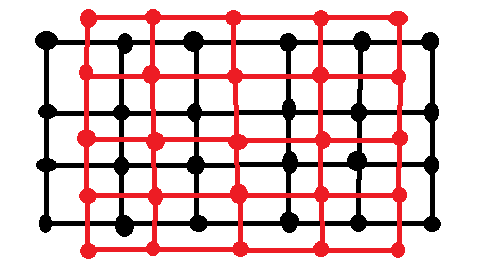
\includegraphics[scale=0.6]{drawings/RectangleDual.png}
	\caption{An example 6 by 4 rectangle R shown in black and the dual $R^h$ in red.}
	\label{fig:rectangle}
\end{figure}

We now prove an important result similar to that of Lemma \ref*{originloop}, for rectangles. Relating the horizontal crossings in primal rectangles to vertical crossings in their duals.

\begin{lemma}
	Let $R$ be a rectangle in $\ints^2$. For any configuration $\omega$ of $\ints^2$, exactly one of the events $H(R)$ and $V^*(R^h)$ holds.
\end{lemma}

\begin{proof}
	WLOG we scale the lattice to avoid working with fractions. Let the lattice $L = (0,2) + 4\ints^2$, and hence its dual $L^* = (2,0)+4\ints^2$. Then let R be a $k$ by $l$ rectangle on $L$ with vertex set $\{(4i,4j+2): 0 \leq i \leq k \text{, } 0 \leq j \leq l-1 \}$
\end{proof}


\section{Conformal Invariance}
Discuss what conformal invariance is and perhaps talk about the result on the triangular lattice due to Smirnov

\section{Simulation}
We discuss various ways of exploring percolation via simulations.
\subsection{The "water level" of open crossings in finite boxes}
{\color{red}{Discuss how uniform R.V.s can be assigned to edges to simulate percolation. 
Then plot the threshold for open crossings across some size box. 
Then see the sharpening of said plot when the box size increases.}}

As we have seen previously the task of determining the percolation threshold for a given lattice structure is highly non-trivial and so for many lattices the task of finding exact values is still an open problem \cite{StoverThreshold}. Subsequently, a great deal of work has been carried out to determine approximate values for a variety of lattices and distributions of open sites or bonds by way of computer simulations. In this section we explore a method I used to estimate the bond percolation threshold for the square lattice, since we can compare this to the exact value of $1/2$ we proved earlier. 

While we know that the fact that a configuration having an open crossing from one side to another of a single finite box in $\ints^2$ does not affect the probability of there being an infinite connected cluster. It is clear that we would expect the probability of such a crossing in a very large box to tend towards the percolation threshold for the infinite cluster. Hence, we can exploit this behaviour to find an estimate for the percolation threshold, create some large square grid, assign some configuration of open and closed edges with probability $p$, then check for a left-right crossing. We alter the value of $p$ repeatedly until we find the lowest value at which a crossing occurs.

There are a number of factors to consider when setting up this simulation such that it can run sufficiently fast, firstly how do we assign each edge to be open or closed so that we can traverse the graph with different values of p.

The simplest approach would be to assign a Bernoulli random variable with probability $p$ to each edge, however this has the drawback of requiring us to revaluate the random variable on each edge when we change the value of $p$, and to mirror the non-decreasing nature of the percolation function $\theta(p)$, we would have to only do this for previously closed edges. To avoid these issues I chose to implement a method similar to one we used to prove \ref{incEventlemma}, where we coupled configurations using uniform random variables. To recap this, by assigning an edge with a value from independent uniform random on $[0,1]$ we can then set an edge to be open if this value is less than or equal to $p$ and closed otherwise. In this way every edge is open with probability $p$, and increasing p has the desired property that edges which were previously open remain so. Additionally, after the values between 0 and 1 have been assigned to each edge, we gain the benefit of only needing to query the state of edges as we come to them by comparing the assigned value to $p$, rather than needing to assign the open or closed states to every edge each time we alter $p$.

We could remove the initial pass of assigning the uniform random variable values to each edge initially. Instead, we could define some hash function mapping the existing attributes of each edge to the range $[0,1]$, allowing us to compute the states of edges on the fly. However, I did not find this speed up necessary.

Secondly how do we check quickly for a given box if there is a left-right crossing. The first step in simplifying this problem to add two auxiliary vertices to the graph, one connected to every vertex on the left-hand side of the box, the other to the right-hand side vertices. Then our problem reduces to whether there is a path between these two auxiliary vertices via open edges.
The fastest way to go about this, since we have an unweighted graph, is to use a version of breadth first search. Taking the subgraph induced by the open edges, note we always set edges incident to the auxiliary edges to be open, we follow a simple algorithm.
\begin{algorithm}
	\caption{Breadth first search from vertex u to v}\label{bfs}
	\begin{algorithmic}[1]
	\Procedure{bfsPath}{$G,u,v$}
	\State{\textbf{Let} $Q$ be a queue}
	\State{\textbf{Let} $explored$ be a list of booleans}
	\State{\textbf{Let} $parent$ be a list of nodes}
	\State{$explored[u] \gets$ True}
	\State{$parent[u] \gets$ None}
	\State $Q$.enqueue($u$)
	\While{$Q$ is not empty}
		\State $x \gets Q\text{.dequeue()}$
		\If {$x$ is $v$} \Comment{Retrace parents to find path}
			\State $path \gets [x]$
			\While{$parent[x]$ is not None}
				\State $path$.prepend(parent[$x$])
				\State $x \gets parent[x]$
			\EndWhile
			\State
			\Return $path$
		\EndIf
		\For{every edge $w$ in $G$.adjacent($x$)}
			\If{$explored[w]$ is False}
				\State $explored[w] \gets$ True
				\State $parent[w] \gets$ $x$
				\State $Q$.enqueue($w$)
			\EndIf
		\EndFor
	\EndWhile
	\If{$explored[v]$ is False}
	 \Return None
	\EndIf
	\EndProcedure
	\end{algorithmic}
	\end{algorithm}

We note a queue is a simple data structure which works in the same way as a queue at a shop. The first item added to the queue is the first to then be removed.
The above algorithm runs in $O(|V|+|E|)$ worst-case time, where $V$ and $E$ are the vertex and edge sets of the graph $G$ respectively. With a little thought it is clear no algorithm can do better for this problem. 

We also note that Algorithm \ref*{bfs} returns the list of nodes on the path between the two vertices. Depending on the use case this can be easily modified to just return true if a path exists. 

Now we can determine if there is a path from one side of a box to another for a given percolation parameter $p$, we want to determine the lowest threshold for which a crossing path exists for a given configuration of uniform random variables. For the case of the planar square lattice we could use some heuristic based on our prior knowledge that the threshold should lie around 1/2. However, to enable the general applicability of the algorithm described to any graph, we do not make any specific assumptions about the threshold distribution.

While a variety of possible approaches exist, a rather efficient one is an adapted form of binary search on the parameter. While usually a binary search can be used to identity sorted items in a list, in some sense our parameter values are also sorted. All the values with a left right crossing appear before those which do have a crossing, this is only true due to our implementation via uniform random variables on each edge.
In order to check if a given value of $p$ is the crossing threshold, we must check a value very close to $p$ to see if it is different. Say we have some precision constant $\epsilon$ then we define:
\begin{itemize}
	\item If $p$ admits a box crossing, then $p$ is the crossing threshold if and only if $p-\epsilon$ does not.
	\item If $p$ does not admit a box crossing, then $p+\epsilon$ is the crossing threshold if and only if $p+\epsilon$ does admit a crossing.
\end{itemize}

Now we can follow an adapted binary search to centre in on the threshold, where we let isPath(G, u, v) be the aforementioned change to Algorithm \ref*{bfs} so that it returns a boolean value.

\begin{algorithm}
	\caption{Find the crossing threshold for a given graph}\label{findthreshold}
	\begin{algorithmic}[1]
	\Procedure{findThreshold}{$G,u,v,\epsilon$} \Comment{u \& v are the auxiliary nodes}
	\State lo $\gets 0$
	\State hi $\gets 1$
	\While{lo $\leq$ hi}
		\State $p \gets (\text{lo}+\text{hi})/2$
		\State openEdges $\gets$ $\{e \in E(G)\text{: e has uniform r.v. value}\leq p\}$
		\State \textbf{let} OpenG be the subgraph of G induced by openEdges
		\If{isPath(openG, u, v)}
			\State altOpenEdges $\gets$ $\{e \in E(G)\text{: unifRV}(e)\leq p-\epsilon\}$
			\State \textbf{let} AltG be the subgraph of G induced by altOpenEdges
			\If{isPath(AltG, u, v)}
				\State hi $\gets p - \epsilon$
			\Else
				\State \Return $p$
			\EndIf
		\Else
			\State altOpenEdges $\gets$ $\{e \in E(G)\text{: unifRV}(e)\leq p+\epsilon\}$
			\State \textbf{let} AltG be the subgraph of G induced by altOpenEdges
			\If{isPath(AltG, u, v)}
				\State \Return $p +\epsilon$
			\Else
			\State lo $\gets p+\epsilon$
			\EndIf
		\EndIf
	\EndWhile
	\EndProcedure
	\end{algorithmic}
\end{algorithm}

You can inspect the above algorithm to see how whenever the current value of $p$ is not the threshold we can safely throw out one half of the current search range. This technique, commonly referred to as divide and conquer, gives good asymptotic search performance. We would say in general a binary search finds the target in $O(nlog(n))$ worst-case time where n is the number of elements to be searched. In our case the effective number of ``items'' depends on the precision parameter $\epsilon$, where the number of potential threshold values to check is $\frac{1}{\epsilon}$. Thus Algorithm \ref*{findthreshold} runs in $O(\frac{1}{\epsilon}log(\frac{1}{\epsilon}))$ worst-case time.

You may notice a possible optimization when both the algorithms are used together. Instead of first constructing the induced subgraph by the open edges then seeing if there is a crossing, we can directly only consider the open edges during our breadth first search by requiring in line 18 of Algorithm \ref*{bfs} that the edges $w$ must have associated uniform random variable value of less than or equal to p. In essence, we can construct the subgraph induced by the open edges on the fly, saving us one pass over the edge set. 

My initial plan to investigate the percolation threshold for the planar square lattice was to simulate many boxes each of increasing width to see how the variation in the crossing threshold decreases with box width. Using the previously described algorithms to find the threshold for each box.

I implemented the simulation using Python due to its extensive set of community libraries and ease of prototyping. Since Python is an interpreted language it can be less performant than other complied languages which can be an important consideration for very large simulations. However, I will later discuss other alternative implementations of Python such as PyPy which can mitigate this issue.
I decided to simulate one box of each width from width 2 (3x3 vertices) to width 1950, with a precision of $0.0001$. I then used the matplotlib library to draw a scatter plot of the box width against the computed crossing threshold, which can be seen in Figure \ref*{fig:thresholdplot2}. The red dashed line lies at the threshold value 0.5 which we know is the true value for an infinite lattice.

You can clearly see how the variability of crossing threshold decreases as the box width increases, becoming more concentrated around 0.5. Supposing we did not already know the true value of the infinite lattice, this would provide us with a strong insight that the percolation threshold lies around 0.5. In fact if we calculate the mean of the crossing thresholds for each box, disregarding the first 50 due to their small size, we would get a value of 0.499979 which when rounded to our precision of 0.0001 is 0.5000.

% \begin{figure}
% 	    \centering
% 	    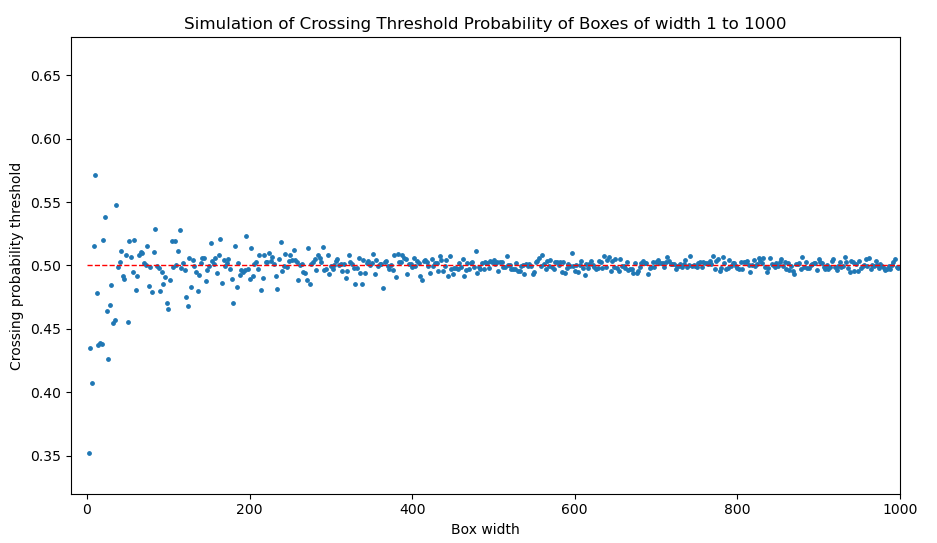
\includegraphics[scale=0.52]{CrossingSimulationPlot2.png}
% 	    \caption{Crossing thresholds for simulated lattices}
% 	    \label{fig:thresholdplot}
% \end{figure}


\begin{landscape}
\begin{figure}
	\centering
	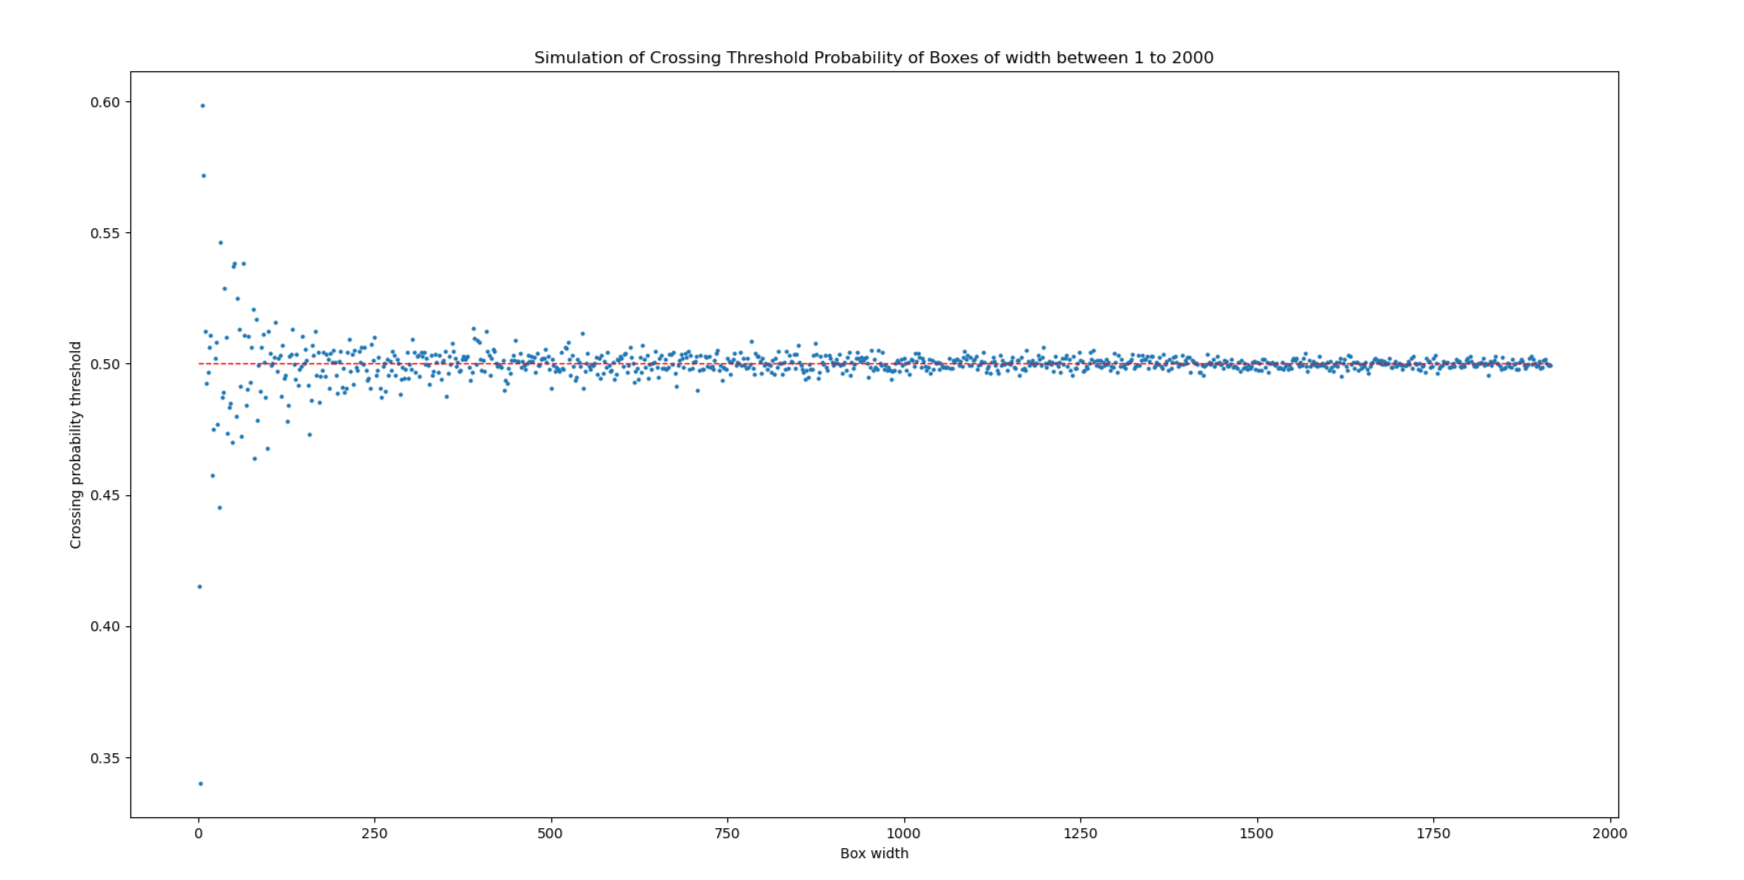
\includegraphics[scale=0.472]{CrossingSimulationPlot3.png}
	\caption{Crossing thresholds for simulated lattices}
	\label{fig:thresholdplot2}
\end{figure}
\end{landscape}
\subsection{Finding the pivotal edges in a finite box}
Discuss an algorithm to find the pivotal edges in the percolation box, perhaps relate to Russo's formula for pivotal edges.
\subsection{Fast Monte Carlo algorithm for percolation}
Discuss the Newman and Ziff paper "A fast Monte Carlo algorithm for site or bond percolation". Explaining the data structures etc, and perhaps implement it.

\section{Conclusion}
Is a conclusion necessary for this project?

% \section{Including maths}

% Some maths, like $\varepsilon>0$ or $a_{23}=\alpha^3$, is written in-line. More important or complex maths is displayed on its own line.
% For example, $$ \lim_{x\to\infty}f(x)=\frac{\pi}{4}.$$

% Sometimes you need multiple lines of maths to line up nicely:

% \begin{align*}
% f(x+y)&=(x+y,-2(x+y))\\
% &=(x,-2x)+(y,-2y)\\
% &=f(x)+f(y),
% \end{align*}

% and sometimes you want to number lines in an equation

% \begin{align}
% A^{T} & =\begin{pmatrix}1 & 2\\
% 3 & 4
% \end{pmatrix}^{T}\\
% \label{my_eqn}  & =\begin{pmatrix}1 & 3\\
% 2 & 4
% \end{pmatrix}
% \end{align}

% \section{References and Figures}
% \LaTeX{} \cite{lamport94} also allows you to cite your sources. For more details on how this can be done, we refer the reader to \cite[sec:~Embedded System]{referencing}. But once you have a bibliography, you can use the cite command easily. Finally we add Figure \ref{fig:logo} to show how to add graphics. Note that we first need to make sure to have the graphic uploaded to Overleaf  or saved in the same folder as your Tex file (whichever is relevant to your case). Notice how the picture was resized using the scale command and that \LaTeX{} determine that the picture looks better above.

% \begin{figure}
%     \centering
%     
\includegraphics[scale=0.6]{uob.pdf}
%     \caption{The logo for the University of Bristol}
%     \label{fig:logo}
% \end{figure}

\printbibliography
% \begin{thebibliography}{99}
% \bibitem{steif}

% % \bibitem{lamport94}
% %   Leslie Lamport,
% %   \textit{\LaTeX: a document preparation system},
% %   Addison Wesley, Massachusetts,
% %   2nd edition,
% %   1994.
  
% % \bibitem{referencing}
% %     Wikibooks,
% %     \textit{\LaTeX/Bibliography Management},
% %     [Online],
% %     Accessed at https://en.wikibooks.org/wiki/LaTeX/Bibliography\_Management,
% %     (DATE ACCESSED).
    

% \end{thebibliography}

\end{document}